% \documentclass[times, twoside, watermark]{zHenriquesLab-StyleBioRxiv}
\documentclass[11pt]{article}
\usepackage{times}
\usepackage[letterpaper,margin=1in]{geometry}
% \usepackage{booktabs}
%\usepackage{lineno}
\usepackage{authblk}
\usepackage{cite}
\usepackage{xr}
\usepackage{xspace}
\usepackage{graphicx}

% To handle cross-referencing between documents
\makeatletter
\newcommand*{\addFileDependency}[1]{% argument=file name and extension
  \typeout{(#1)}
  \@addtofilelist{#1}
  \IfFileExists{#1}{}{\typeout{No file #1.}}
}
\makeatother

\newcommand*{\myexternaldocument}[1]{%
    \externaldocument{#1}%
    \addFileDependency{#1.tex}%
    \addFileDependency{#1.aux}%
}

\myexternaldocument{extra_insight_manuscript}

\renewcommand{\baselinestretch}{1.5} % line spacing
\setlength{\parskip}{1em} % paragraph spacings
\renewcommand\Authfont{\fontsize{10}{10}\selectfont} % author font size
\renewcommand\Affilfont{\fontsize{9}{9}\selectfont} % affil font size

\linespread{1.15}
\title{Supplemental Material for: Global characterization of mutations of large
  selective effect in the human genome}
%\title{Non-coding ultra-strong selection in the human genome varies by regulatory role and phylogenetic conservation}
%\leadauthor{Dukler}
%\shorttitle{ExtRaINSIGHT}
\author[1]{Noah Dukler}
\author[1]{Mehreen R. Mughal}
\author[2]{Yi-Fei Huang}
\author[1]{Adam Siepel}

\linespread{1.15}
\affil[1]{Simons Center for Quantitative Biology, Cold Spring Harbor Laboratory, Cold Spring Harbor, NY}
\affil[2]{Department of Biology and Huck Institutes of the Life
  Sciences, University Park, PA}
\date{}

\begin{document}

\maketitle{}


%%%%%%%%%%%%%%%%%%%%
%% IMPORTANT: create all labels here with an S prefix so that prettyref can format them correctly in the main doc.
%% Currently implemented prefixes are: Sfig. See the header of the main doc to add more.
%%%%%%%%%%%%%%%%%%%%

\section*{Supplemental Figures}

\begin{figure}
    \centering
    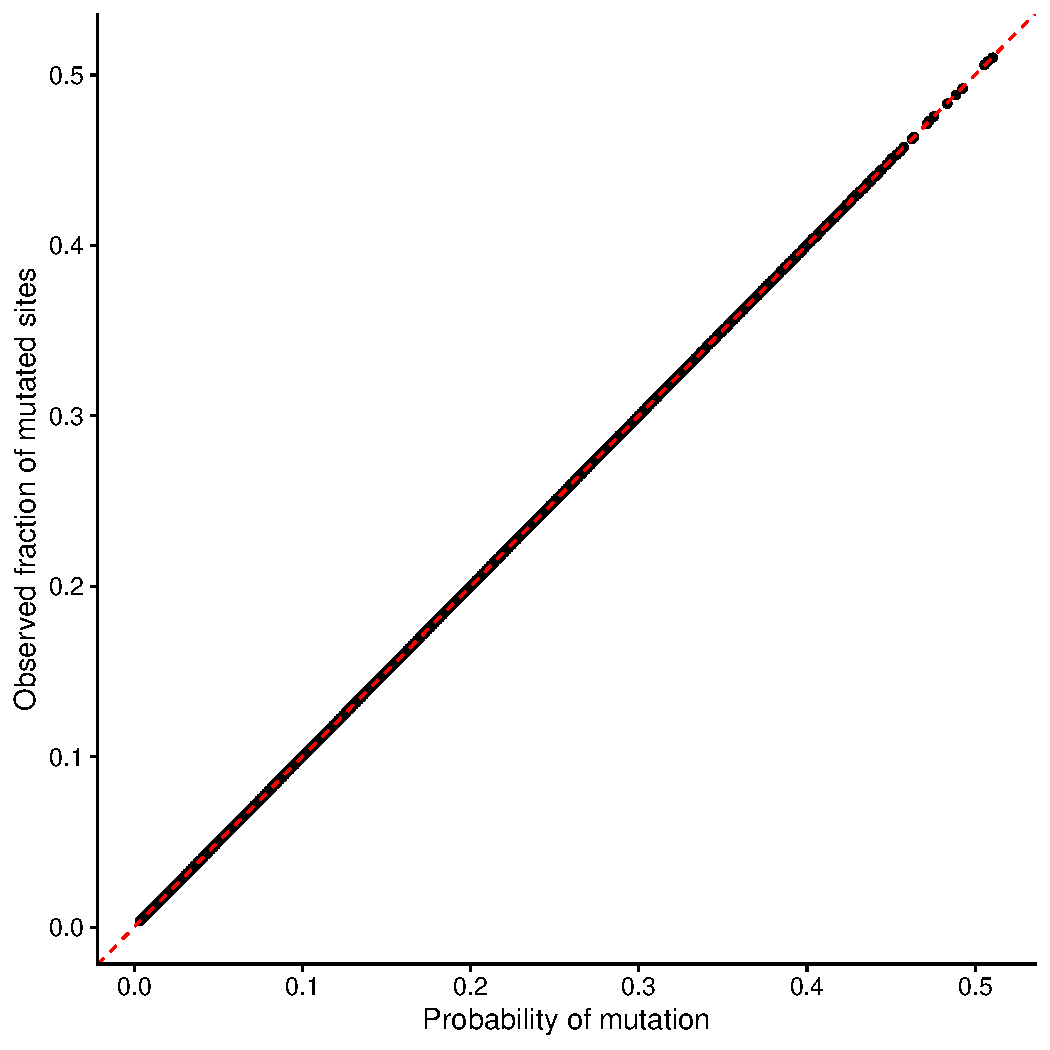
\includegraphics[width = 0.5\linewidth]{supplemental_figures/mutation_model_calibration.pdf}
    \caption{\textbf{The mutation model is globally well calibrated in neutral regions}}
    \label{Sfig:mutation_model_calibration}
\end{figure}

\begin{figure}[t]
    \centering
    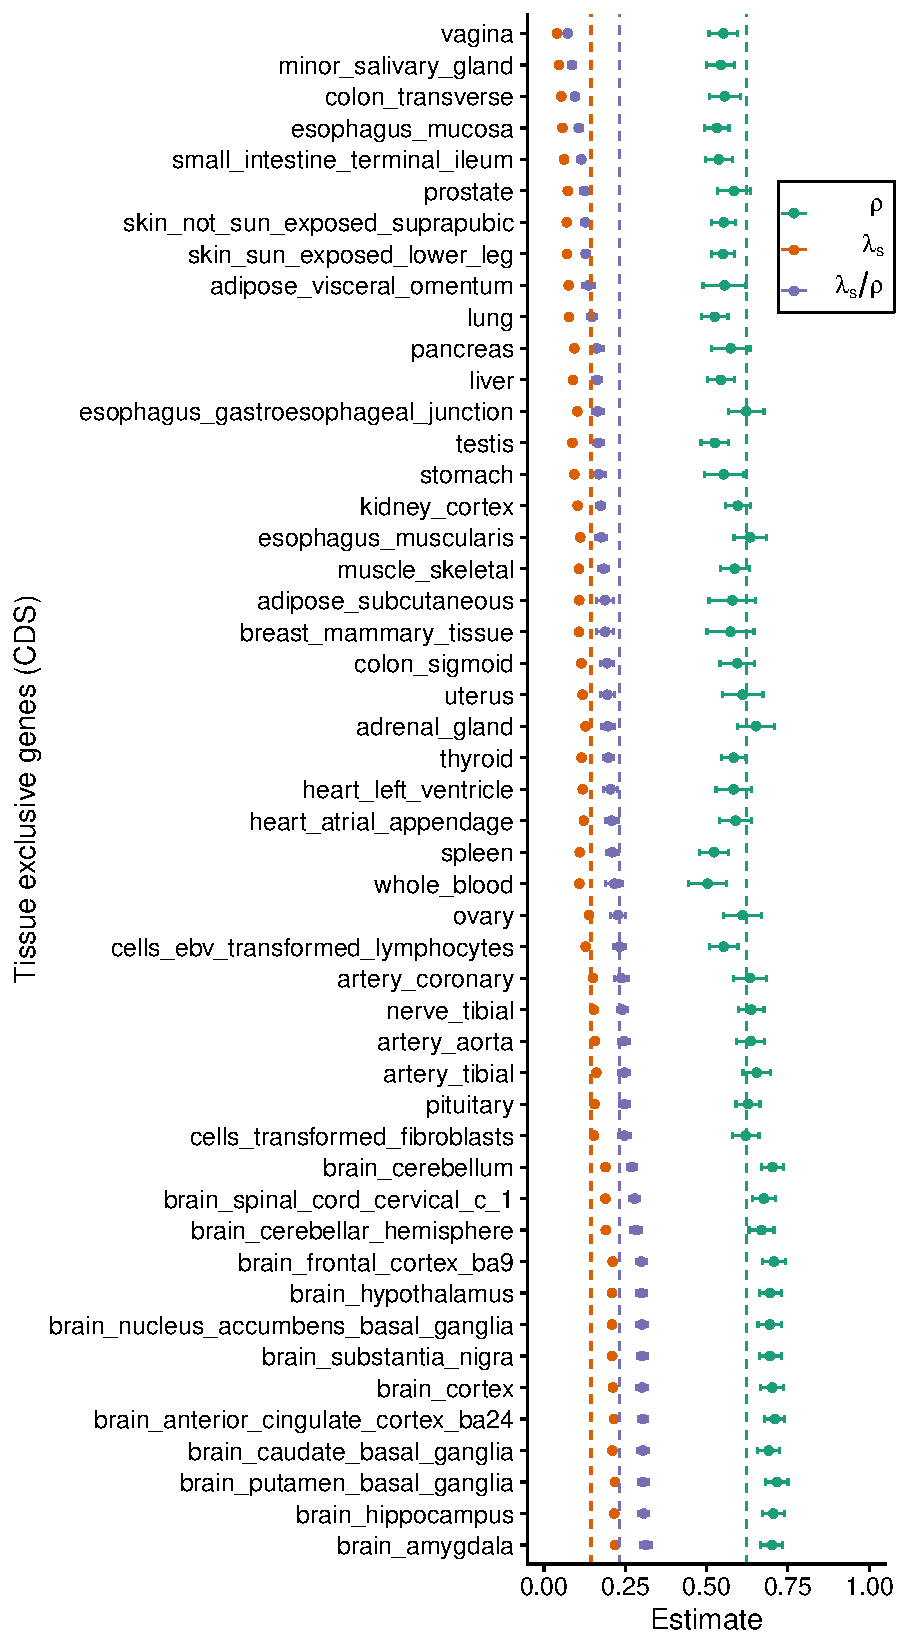
\includegraphics[width=0.6\linewidth]{supplemental_figures/tissue_specificity_cds_ratio.pdf}
    \caption{\textbf{ExtRaINSIGHT scores in CDS of tissue-specific genes}}
    \label{Sfig:tissue_specific_scores}
\end{figure}

\end{document}

